\section{Poisson Recommendation}
\label{sec:model}

% !!! review the Gamama and Poisson near the generative process.
% !!! make n_u and n_i the sums
% !!! somewhere we need to make clear how our notation works

In this section we describe the Poisson factorization model for
recommendation, and discuss its statistical properties.

We are given data about users and items, where each user has consumed
and possibly rated a set of items.  The observation $y_{ui}$ is the
rating that user $u$ gave to item $i$, or zero if no rating was given.
(In so-called ``implicit'' consumer data, $y_{ui}$ equals one if user
$u$ consumed item $i$ and zero otherwise.)  User behavior data, such
as purchases, ratings, clicks, or views, are typically sparse.  Most
of the values of the matrix $y$ are zero.

We model the data with factorized Poisson
distributions~\cite{Canny:2004}.  We represent each item $i$ as a
vector of $K$ latent attributes $\beta_i$ and represent each user $u$
as a vector of $K$ latent preferences $\beta_u$.  These vectors are
sparse and non-negative.  The observations $y_{ui}$ are modeled with a
Poisson, parameterized by the inner product of the user preferences
and item attributes, $y_{ui} \sim \poisson(\theta_u^\top \beta_i)$.
This is a variant of probabilistic matrix
factorization~\cite{Salakhutdinov:2008a} but where each user and
item's weights are positive~\cite{Lee:1999} and where the Poisson
replaces the Gaussian.

Beyond the basic data generating distribution, we place Gamma priors
on the latent attributes and latent preferences, which encourage the
model towards sparse representations of the users and items.
Furthermore, we place additional priors on the user and item-specific
scale parameter of those Gammas, which controls the average size of
the representation.  This hierarchical structure allows us to capture
the diversity of users, some tending to consume more than others, and
the diversity of items, some being more popular than others.  The
literature on recommendation systems suggests that a good model must
capture such heterogeneity across users and items~\cite{Koren:2009}.

Putting this together, the generative process of the hierarchical
Poisson factorization model (HPF) is as follows:
\begin{enumerate*}
\item For each user $u$:
  \begin{enumerate*}
  \item Sample activity $\xi_u \sim \gam(a', a'/b')$.
  \item For each component $k$, sample preference $$\theta_{uk} \sim
    \gam(a, \xi_u).$$
  \end{enumerate*}

\item For each item $i$:
  \begin{enumerate*}
    \item Sample popularity $\eta_i \sim \gam(c', c'/d')$.
    \item For each component $k$, sample attribute
      $$\beta_{ik} \sim \gam(c, \eta_i).$$
  \end{enumerate*}

\item For each user $u$ and item $i$, sample rating
  $$y_{ui} \sim
  \poisson(\theta_u^\top \beta_i).$$
\end{enumerate*}
This process describes the statistical assumptions behind the model.
Note that we also study a sub-class of the HPF where we fix the rate
parameters for all users and items to the same pair of
hyperparameters. We call this model Bayesian Poisson Factorization
(BPF).

The central computational problem is posterior inference, which is
akin to ``reversing'' the generative process.  Given a user behavior
matrix, we want to estimate the conditional distribution of the latent
per-user and per-item structure, $p(\theta_{1:N} \beta_{1:M} \g y)$.
The posterior is the key to recommendation.  We estimate the posterior
expectation of each user's preferences, each items attributes and,
subsequently, form predictions about which unconsumed items each user
will like.  We discuss our posterior inference algorithm in detail in
\mysec{inference}.  Figure 1 illustrates posterior estimates of
$\beta$ and $\theta$ on Netflix data.

% jmh: the below seemed out of place, and is repeated in the algorithm
% section just before empirical results, which seems like a better
% spot

%% \subsection{The Posterior distribution}
%% The posterior distribution of the latent variables $p(\theta, \beta,
%% \xi, \eta \g y)$ embeds users and items in a latent space of
%% $K$-dimensional positive vectors. 

%% We use the HPF to recommend items to users by predicting which of the
%% unconsumed items each will like.  We rank each user's unconsumed items
%% by their posterior expected Poisson parameters,
%% \begin{equation}
%%   \label{eq:score}
%%   \textrm{score}_{ui} = \E[\theta_u^\top \beta_i \g y].
%% \end{equation}
%% This amounts to asking the model to rank by probability which of the
%% presently unconsumed items each user will likely consume in the
%% future.

\subsection{Properties of HPF}

With the modeling details in place, we highlight several statistical
properties of hierarchical Poisson factorization.  These properties
provide advantages over classical (Gaussian) matrix
factorization.~\footnote{Classical matrix factorization is L2
  regularized matrix factorization with bias terms for users and
  items, fit using stochastic gradient descent~\cite{Koren:2009}. Without the bias terms,
  this corresponds to maximum a-posteriori inference under
  Probabilistic Matrix Factorization~\cite{Salakhutdinov:2008a}.}
{\bf HPF captures sparse factors}.  As we mentioned above, the Gamma
priors on preferences and attributes encourages sparse representations
of users and items.  Specifically, by setting the shape parameter $a$
to be small, most of the weights will be close to zero and only a few
will be large.

% dmb: !!! above, cite something for this property.  without even
% looking at it, citing johnson and kotz (continuous multivariate
% distributions) is probably safe.

{\bf HPF models the long-tail of users and items}.  One statistical
characteristic of real-world user behavior data is the distribution of
user activity (i.e., how many items a user consumed) and item
popularity (i.e., how many users consumed an item).  These
distributions tend to be long-tailed: while most users consume a
handful few items, a few ``tail users'' consume thousands of items.  A
question we can ask of a statistical model of user behavior data is
how well it captures these distributions.  We found that HPF captures
them very well, while classical matrix factorization does not.

To check this, we implemented a visual \textit{posterior predictive
  check}~\cite{Rubin:1984,Gelman:1996} (PPC), a technique for model
assessment from the Bayesian statistics literature.  The idea behind a
PPC is to simulate a complete data set from the posterior predictive
distribution, the distribution over data that the posterior induces,
and then compare the generated data set to the true observations in
relevant ways.  A good model will produce data that captures the
important characteristics of the observed data.

We developed a PPC for matrix factorization algorithms on user
behavior data.  First, we formed posterior estimates of user
preferences and item attributes for both classical MF and HPF.  Then,
from these estimates, we generated a new user behavior matrix by
drawing values for each user and item.  (For classical matrix
factorization, we truncated these values at zero and rounded to one in
order to generate a plausible matrix.)  Finally, we visually compared
the matrix generated by the posterior predictive distribution to the
true observations.

\myfig{marginals} illustrates our PPC for the Netflix data.  In this figure, we
illustrate three distributions over user activity: the observed
distribution (squares), the distribution from a data set replicated by
HPF (red line), and a distribution from a data set replicated by
classical MF (blue line).  HPF captures the truth much more closely
than classical MF, which badly overestimates the distribution of user
activity.  (We note that this is true for the item popularities as
well, and for the other data sets.) This indicates that HPF gives
better fit to real data when measured by its ability to capture
distributions of user activity and item popularity.

% Figure 3 shows the distributions of user activity on large,
% real-world ratings data sets. Under the BPF and the HPF, the
% marginal distribution of each user's ratings, with the item weights
% held fixed, is a negative binomial.  Let $y_{u} = \sum_{i} y_{ui}$
% be the sum of the ratings for user $u$.  Since each of the terms in
% the sum is a Poisson distribution with rate $\theta_u^\top \beta_i$,
% the sum is itself a Poisson random variable~\cite{Johnson:2005}.
% \begin{equation}
%   y_u \sim \poisson\left(\theta_u^\top (\textstyle \sum_{i} \beta_{i})\right).
% \end{equation}
% Holding the item weights fixed, note that the rate of this Poisson
% is a sum of scaled Gamma random variables $\beta_{ik} \theta_{uk}$,
% which is itself a Gamma variable~\cite{Norman:1994}.  Thus the
% marginal distribution of $y_u$ is from an integrated Gamma-Poisson
% distribution, which is a negative binomial~\cite{Gelman:1995}.

% The negative binomial is a long-tailed distribution that is known to
% fit user activity well~\cite{Goodhardt:1984,Dunning:1993}.  Figure 3
% shows that the HPF provides good fits to the distribution of user
% activity on real-world data.  Classical matrix factorization is
% based on Gaussian likelihoods, and the marginal distribution of
% total user ratings is a Gaussian.  The Gaussian is a poor choice for
% modeling long-tailed distributions. Further, it places probability
% mass on negative numbers, a setting that never occurs. While we have
% focused on user activity here, the same is true for the marginal
% distribution of item popularities under Poisson factorization.

\begin{figure}[t!]
  \centering
  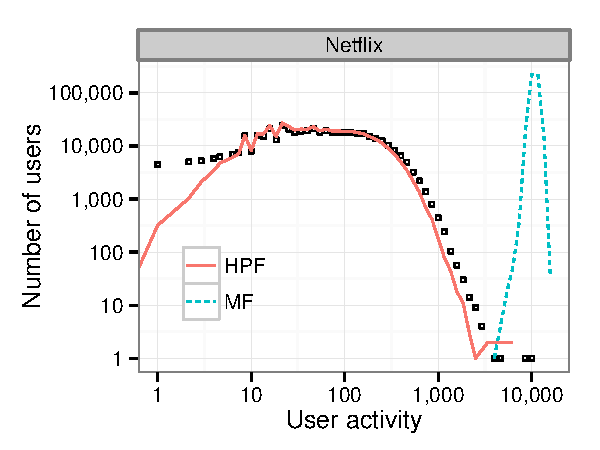
\includegraphics[width=0.4\textwidth]{figures/user_activity_sim_netflix.pdf}
  \caption{The distribution of total ratings for the Netflix dataset.
    The pink curve shows the empirical count of the number of users
    who have rated a given number of items, while the green and blue
    curves show the simulated totals from fitted Poisson and
    traditional matrix factorization models, respectively. The Poisson
    marginal closely matches the empirical, whereas classical matrix
    factorization fits a large mean to account for skew in the
    distribution and the missing ratings.}
\label{fig:marginals}
\end{figure}

{\bf HPF downweights the effect of zeros.}  Another advantage of HPF
is that it implicitly down-weights the contribution of the items that
each user did not consume.  With an appropriate fit to user activity,
the model has two ways of explaining an unconsumed item: either the
user is not interested in it or she would be interested in it but is
likely to not be further active. In contrast, a user that consumes an
item must be interested in it.  Thus, the model benefits more from
making a consumed user/item pair more similar than making an
unconsumed user/item pair less similar.

Classical MF is based on Gaussian likelihoods (i.e., squared loss),
which gives equal weight to consumed and unconsumed items.
Consequently, when faced with a sparse matrix and implicit feedback,
i.e., binary consumption data, matrix factorization places more total
emphasis on the unconsumed user/item pairs.  (This too can be seen to
stem from classical MF's overestimation of the distribution of user
activity.)  To address this, researchers have patched the model in
complex ways, for example, by including per-observation
confidences~\cite{Koren:2009} or considering all zeroes to be hidden
variables~\cite{Paquet:2013p9197}.  Poisson factorization more
naturally solves this problem by better capturing each user's rate of
consumption.

As an example, consider two similar science fiction movies, ``Star
Wars'' and ``The Empire Strikes Back'', and consider a user who has
seen one of them.  The Gaussian model pays an equal penalty for making
the user similar to these items as it does for making the user
different from them---with quadratic loss, seeing ``Star Wars'' is
evidence for liking science fiction, but not seeing ``The Empire
Strikes Back'' is evidence for disliking it.  The Poisson model,
however, will prefer to bring the user's latent weights closer to the
movies' weights because it favors the information from the user
watching ``Star Wars''. Further, because the movies are similar, this
increases the Poisson model's predictive score that a user who watches
``Star Wars'' will also watch ``The Empire Strikes Back''.

{\bf Fast inference with sparse matrices.}  Finally, the likelihood of
the observed data under HPF (and BPF) depends only on the consumed
items, that is, the non-zero elements of the user/item matrix $y$.
This facilates computation for the kind of sparse matrices that we
tend to observe in real-world data.

We can see this property from the form of the Poisson distribution.
Given the latent preferences $\theta_u$ and latent attributes
$\beta_i$, the Poisson distribution of the rating $y_{ui}$ is
\begin{equation}
  p(y_{ui} \g \theta_u, \beta_i) =
  \left(\theta_u^\top \beta_i\right)^y
  \exp\left\{-\theta_u^\top \beta_i \right\} / y_{ui}!
\end{equation}
Recall the elementary fact that $0! = 1$.  The log probability of the
complete matrix $y$ is
\begin{align}
  \log p(y \g \theta, \beta) =
  & \left(\textstyle \sum_{\{y_{ui} > 0\}}
    y_{ui} \log (\theta_u^\top \beta_i) - \log y_{ui}!
  \right) \\
  & -
  \left(\textstyle\sum_{u} \theta_u\right)^\top \left(\textstyle
    \sum_{i} \beta_i\right). \nonumber
\end{align}

Classical MF does not enjoy this property. These methods, especially
when applied to massive data sets of implicit feedback, must (in
theory) iterate over all the cells of the matrix.  Practitioners
require solutions such as sub-sampling~\cite{Dror:2012a}
approximation~\cite{Hu:2008p9402}, or stochastic
optimization~\cite{Mairal:2010}.
